%% Section 1
\section{Introduction}
\label{sec:introduction}
A class imbalanced dataset refers to a dataset in which the ratios of data belonging to different classes are not equal but are skewed to one side.
Imbalanced data is a problem that is commonly encountered in data classification using machine learning (ML).
When training is conducted in a state of imbalanced data distribution, the ML-based classifier has a limitation characterized by over-fitting the data of a class with a high proportion in the training data.
When the data are skewed to one side, the classifier is highly likely to misclassify the data belonging to the minority class by comparing it with the data belonging to the majority class.\\
A typical strategy for processing imbalanced data is the synthetic minority oversampling technique (SMOTE)~\cite{DBLP:journals/jair/ChawlaBHK02}.
SMOTE is a technique that intelligently expands the data of the minority class and shows better classification performance than the oversampling technique using simple replication.
Recently, there have been various studies on generative adversarial networks (GANs)~\cite{DBLP:conf/gecco/ChoK19}, and data sampling has been attempted using GANs, in addition to SMOTE, thereby improving classifier performance~\cite{DBLP:conf/iciss/GangwarR19}.
However, many experiments and tests should be conducted to improve the classification performance by adjusting the ratio of classes.
Such a process may be difficult and inefficient.
Study was conducted to find the optimal SMOTE ratio by using the support vector regression (SVR) technique, and the results were better than those of previous methods~\cite{DBLP:journals/cin/SeoK18}.
In this study, a genetic algorithm (GA) is used to search for various combinations of oversampling ratios based on the SMOTE and GAN techniques and to improve the performances of classifiers.\\
This paper is organized as follows: in Section~\ref{sec:ga}, the proposed GA-based oversampling ratio optimization method is explained, and in Section~\ref{sec:experiments-results}, the experiments and results are discussed. Finally, the paper is concluded in Section~\ref{sec:conclusion}.


%% Section 2
\section{Genetic Algorithm}
\label{sec:ga}
\textbf{Encoding:} a chromosome refers to a combination of oversampling ratios obtained using various techniques.
Each gene of a chromosome indicates how much oversampling will be done using either the SMOTE or GAN technique, i.e., the sampling ratio for each technique.\\
\textbf{Fitness:} the fitness of each chromosome is calculated using the performance of a trained classifier.
The data of the minority class in the training dataset are oversampled according to the combination represented by the chromosome, and the classifier is trained using the sampled dataset.
The performance of the trained classifier is evaluated using the training dataset, and the $\emph{F}_{1}$ score, which is an evaluation metric, is used for fitness.\\
\textbf{Selection:} we use the Roulette wheel method, which is the most representative selection method.\\
\textbf{Crossover:} since a chromosome is a one-dimensional array with a certain length, a one-point crossover, which exchanges the chromosomes of parents at an arbitrary point, is used as the crossover operator.\\
\textbf{Mutation:} two arbitrary points are chosen in the chromosome, and the mutation operator is used to exchange the genes at the two points.
In other words, two techniques are selected, and the oversampling ratios of these techniques are exchanged.\\
\textbf{Replacement}: the replacement operator is used to maintain population diversity through an operation that replaces the parents with the offspring.

\begin{figure}[t]
    \centering
    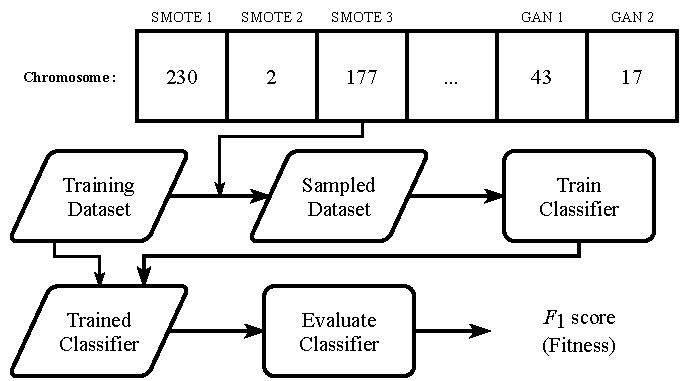
\includegraphics[width=\columnwidth]{figure-1.pdf}
    \caption{Example of fitness calculation}
    \label{fig:1}
\end{figure}


%% Section 3
\section{Experiments and Results}
\label{sec:experiments-results}
We used a credit card fraud detection dataset in the experiments.
This dataset is one of the representative class imbalanced datasets, and includes credit card transactions that were carried out in Europe for two days in September, 2013.
The total number of datasets is 284,807; out of these 284,315 are normal transactions while 492 are fraud transactions.
In the experiments, 75\% of the total data was used as the training dataset while the remaining 25\% was used to evaluate the trained model.\\
We used a deep-neural network (DNN)-based classifier in the experiment.
The number of hidden layers in the neural network is 2, and the number of nodes in the hidden layer is 20 and 11.
The neural network was implemented using \emph{PyTorch}\footnote{https://pytorch.org/}.\\
A total of 13 oversampling strategies with different parameters were used to increase the volume of data in the minority class in the experiments.
The strategies can be divided into three main types: oversampling strategies using $\emph{k}$-NN-based SMOTE, SVM algorithm-based SMOTE, and GAN.
Specifically, there are three oversampling strategies that use the $\emph{k}$-NN-based SMOTE, eight that use the SVM algorithm-based SMOTE, and two that use the GAN.
The SMOTE strategies were provided by \emph{Imbalanced-Learn}\footnote{https://imbalanced-learn.readthedocs.io/}, and the GAN was implemented using \emph{PyTorch}.\\
As described above, a total of 13 oversampling strategies were developed, and using the GA, we conducted experiments to investigate how to set and combine the oversampling ratios of each technique to find the optimal combination.
The following parameters of GA were used: the length of each chromosome was 13, and the sum of all genes of each chromosome was initialized to be between 381 and 1,524.
Each generation had a population size of 128, and a total of 100 generations were searched.
Furthermore, 16 parents were selected in each generation and 16 offspring were transferred to the next generation.
The probability of mutation was 1\%.
The performance of the trained classifier was compared with that of a classifier trained by oversampling with the optimal combination searched using the GA, and that of a classifier trained by oversampling using a strategy characterized by a certain ratio (the ratio was set to $200\%$ with an increase of 381, 300\% with an increase of 762, 400\% with an increase of 1143, and 500\% with an increase of 1,524).
Our code for this paper and experiment is on \emph{GitHub}\footnote{https://github.com/hwyncho/GECCO-2020-PyTorch.git/}.\\
As described in Section~\ref{sec:ga}, we evaluated the trained classifier with the training dataset and calculated the $\emph{F}_{1}$ score as the fitness.
Table~\ref{tab:1} shows the results of comparing the $\emph{F}_{1}$ scores of the scenario where the imbalanced dataset was trained, that in which 13 techniques with four fixed ratios were used, and that in which the data sampled was trained with a ratio optimized using the GA.
When the GA was used, the performance was better than those in all other cases.

\begin{table}[t]
    \centering
    \caption{Results for each oversampling strategy}
    \begin{tabular}{c|c|c|c}
        \toprule
        \multicolumn{2}{c|}{\textbf{Case}} & \textbf{$\emph{F}_{1}$ score} & \textbf{Std.} \\
        \hline
        \multirow{2}{*}{Imbalanced} & Train & 0.8271 & $NA$ \\
        & Evaluate & 0.7797 & $NA$ \\
        \hline
        Single strategy & Train & 0.8929 & 0.045 \\
        (42 cases) & Evaluate & 0.8553 & 0.0373 \\
        \hline
        \multirow{2}{*}{Proposed strategy} & Train & \textbf{0.9822} & $NA$ \\
        & Evaluate & \textbf{0.8895} & $NA$ \\
        \bottomrule
    \end{tabular}
    \label{tab:1}
\end{table}


%% Section 4
\section{Conclusion}
\label{sec:conclusion}
In this study, we used the GA to explore and optimize the combination of oversampling ratios for each strategy using SMOTE and GAN.
A comparison was made between the proposed method and the case in which the class imbalanced dataset was trained, and the one in which training was conducted using a single technique with oversampled data at a certain ratio.
As a result, the classifier that learned the oversampled data with a ratio optimized using the proposed method was superior in classification performance in every case.
Through this method, we confirmed the possibility of optimizing the combination of oversampling ratios.